\documentclass{book}

%------------------------------------ Packages ------------------------------------
%\usepackage[utf8]{inputenc}
\usepackage{graphicx}
\usepackage{nomencl}
\usepackage{amssymb}
\usepackage{amsmath}
\usepackage[english]{babel}
\usepackage[ddmmyyyy]{datetime}
\usepackage{hyperref}
\usepackage[style=nature,backend=bibtex,maxbibnames=99]{biblatex}
\usepackage{csquotes}
\usepackage[a4paper,lmargin={2.5cm},rmargin={2.5cm},tmargin={2.5cm},bmargin = {2.5cm}]{geometry}
\usepackage{epigraph}
\usepackage[nopostdot,nogroupskip,style=super,nonumberlist,toc,automake,toc]{glossaries}
\usepackage{titlesec}
\usepackage[most]{tcolorbox}
\usepackage[font=small,labelfont=bf]{caption}
\usepackage{titlesec}
\usepackage{tikz}
\usetikzlibrary{mindmap}

%------------------------------------ Settings ------------------------------------
% references
\addbibresource{literature.bib} 
\newcommand{\Chapref}[1]{\hyperref[#1]{Chapter~\ref*{#1}}} % capitalize link to chapter

% figures
\graphicspath{{figures/}}
\captionsetup[figure]{font=small,justification=raggedright,singlelinecheck=false}
\newcommand{\dummyfig}[1]{
  \centering
  \fbox{
    \begin{minipage}[c][0.33\textheight][c]{0.5\textwidth}
      \centering{#1}
    \end{minipage}
  }
}

% section numbers
\setcounter{tocdepth}{2}
\setcounter{secnumdepth}{2}
% \titlespacing{\subsubsection}{0pt}{\parskip}{-\parskip}

% color
\hypersetup{colorlinks=true,
linkcolor=black,
filecolor=magenta,
urlcolor=black
}


% line spacing
\renewcommand{\baselinestretch}{1.5}

% footnotes
\renewcommand{\footnotesize}{\fontsize{10}{12}\selectfont}


%------------------------------------ Abbreviations -------------------------------
\makeglossaries

%Here we define a set of example acronyms

%%%%%%%%%%%%%%%%%%%%%%%%%% A %%%%%%%%%%%%%%%%%%%%%%%%%%
\newacronym{ai}{AI}{artificial intelligence}

%%%%%%%%%%%%%%%%%%%%%%%%%% B %%%%%%%%%%%%%%%%%%%%%%%%%%
\newacronym{bci}{BCI}{brain computer interface}

%%%%%%%%%%%%%%%%%%%%%%%%%% C %%%%%%%%%%%%%%%%%%%%%%%%%%
\newacronym{crunch}{CRUNCH}{compensation-related utilization of neural circuits hypothesis}
\newacronym{cnn}{CNN}{convolutional neural network}
\newacronym{csp}{CSP}{common spatial patterns}
%%%%%%%%%%%%%%%%%%%%%%%%%% D %%%%%%%%%%%%%%%%%%%%%%%%%%
\newacronym{dmd}{DMD}{dynamic mode decomposition}
\newacronym{dmn}{DMN}{default mode network}

%%%%%%%%%%%%%%%%%%%%%%%%%% E %%%%%%%%%%%%%%%%%%%%%%%%%%
\newacronym{ecog}{ECoG}{electrocorticography}
\newacronym{eeg}{EEG}{electroencephalography}
\newacronym{erm}{ERM}{empirical risk minimization}
\newacronym{erp}{ERP}{event related potential} 
%%%%%%%%%%%%%%%%%%%%%%%%%% F %%%%%%%%%%%%%%%%%%%%%%%%%%
\newacronym{fmri}{fMRI}{functional magnetic resonance imaging}

%%%%%%%%%%%%%%%%%%%%%%%%%% G %%%%%%%%%%%%%%%%%%%%%%%%%%
%%%%%%%%%%%%%%%%%%%%%%%%%% H %%%%%%%%%%%%%%%%%%%%%%%%%%
\newacronym{harold}{HAROLD}{hemispheric asymmetry reduction in older adults}
%%%%%%%%%%%%%%%%%%%%%%%%%% I %%%%%%%%%%%%%%%%%%%%%%%%%%
\newacronym{ica}{ICA}{independent component analysis}
%%%%%%%%%%%%%%%%%%%%%%%%%% J %%%%%%%%%%%%%%%%%%%%%%%%%%
%%%%%%%%%%%%%%%%%%%%%%%%%% K %%%%%%%%%%%%%%%%%%%%%%%%%%
%%%%%%%%%%%%%%%%%%%%%%%%%% L %%%%%%%%%%%%%%%%%%%%%%%%%%
\newacronym{lda}{LDA}{linear discriminant analysis}
%%%%%%%%%%%%%%%%%%%%%%%%%% M %%%%%%%%%%%%%%%%%%%%%%%%%%
\newacronym{mvpa}{MVPA}{multivariate pattern analysis}
\newacronym{mle}{MLE}{maximum likelihood estimation}
\newacronym{mri}{MRI}{magnet resonance imaging}
%%%%%%%%%%%%%%%%%%%%%%%%%% N %%%%%%%%%%%%%%%%%%%%%%%%%%
%%%%%%%%%%%%%%%%%%%%%%%%%% O %%%%%%%%%%%%%%%%%%%%%%%%%%
%%%%%%%%%%%%%%%%%%%%%%%%%% P %%%%%%%%%%%%%%%%%%%%%%%%%%
\newacronym{pasa}{PASA}{posterior–anterior shift in aging}
\newacronym{pca}{PCA}{principal component analysis}
\newacronym{pet}{PET}{positron emission tomography}
%%%%%%%%%%%%%%%%%%%%%%%%%% Q %%%%%%%%%%%%%%%%%%%%%%%%%%
%%%%%%%%%%%%%%%%%%%%%%%%%% R %%%%%%%%%%%%%%%%%%%%%%%%%%
\newacronym{rf}{RF}{random forest}
%%%%%%%%%%%%%%%%%%%%%%%%%% S %%%%%%%%%%%%%%%%%%%%%%%%%%
\newacronym{stac}{STAC}{scaffolding theory of cognitive aging}
\newacronym{svm}{SVM}{support vector machine}
%%%%%%%%%%%%%%%%%%%%%%%%%% T %%%%%%%%%%%%%%%%%%%%%%%%%%
\newacronym{tsne}{t-SNE}{t-distributed stochastic neighbor embedding}
%%%%%%%%%%%%%%%%%%%%%%%%%% U %%%%%%%%%%%%%%%%%%%%%%%%%%
\newacronym{umap}{UMAP}{uniform manifold approximation and projection for dimension reduction}
\newacronym{un}{UN}{United Nations}
%%%%%%%%%%%%%%%%%%%%%%%%%% V %%%%%%%%%%%%%%%%%%%%%%%%%%
%%%%%%%%%%%%%%%%%%%%%%%%%% W %%%%%%%%%%%%%%%%%%%%%%%%%%
\newacronym{who}{WHO}{World Health Organization}

%%%%%%%%%%%%%%%%%%%%%%%%%% X %%%%%%%%%%%%%%%%%%%%%%%%%%
%%%%%%%%%%%%%%%%%%%%%%%%%% Y %%%%%%%%%%%%%%%%%%%%%%%%%%
%%%%%%%%%%%%%%%%%%%%%%%%%% Z %%%%%%%%%%%%%%%%%%%%%%%%%%
%------------------------------------ Document ------------------------------------
\begin{document}
%---------------------------------- Title Page -----------------------------------
\begin{titlepage}
    \begin{center}
        \vspace*{1cm}
        \Huge
        \textbf{WORKING TITLE: Using machine learning aging neuroscience}
                        
        \vspace{1.5cm}
        \LARGE
        By\\
        \vspace{0.5cm}
        \textbf{Christian Johannes Gölz\\}
        \vspace{0.5cm}       
        A thesis presented for the degree of\\
        Doctor rerum naturalium\\
        (Dr. rer. nat)
        \vfill
        \Large
        Paderborn University\\
        Faculty of natural sciences\\
        2022
            
    \end{center}
\end{titlepage}



\tableofcontents

\chapter*{Acknowledgement}
\addcontentsline{toc}{chapter}{Acknowledgement}
\vspace*{\fill}
\begin{center}
Danke.
\end{center}
\vspace*{\fill}

\chapter*{Abstract}
\addcontentsline{toc}{chapter}{Abstract}
\setcounter{page}{3}
Aim: Apply data science methods to questions in aging Neuroscience\\
Methods: Supervised and unsupervised methods in different settings\\
Results: Novel Data Driven insights\\
Coclusion: ML rocks!

\chapter*{Figures}
\addcontentsline{toc}{chapter}{Figures}

\chapter*{Tables}
\addcontentsline{toc}{chapter}{Tables}

\printglossary[title={List of Abbreviations}]

\chapter*{Publications and other scientific contributions}
\addcontentsline{toc}{chapter}{Publications and other scientific contributions}
\fullcite{Goelz2021a}\\
\\
\fullcite{Goelz2023}\\
\\
\fullcite{Goelz2021b}\\
\\
\twocite{Gaidai2022}\\
\\
\fullcite{Goelz2018}\\
\\
\fullcite{vieluf2018age}\\
\\
\fullcite{Ströhlein2020}\\
\\
\fullcite{Gowik2023}\\
\\
\fullcite{Strote2020}\\
\\
\fullcite{Strote2020}\\
\\
\fullcite{Niess2022}

\chapter{General Introduction}\label{chap:intro}
\pagenumbering{arabic}

    \section{Motivation}
    \setlength{\epigraphwidth}{0.6\textwidth}
\epigraph{\centering "Humans now live longer than at any time in history. But adding more years to life can be a mixed blessing if it is not accompanied by adding more life to years."} {Dr. Tedros Adhanom Ghebreyesus, WHO Director-General, 2020}

\noindent One of the major societal challenges facing Western societies is the demographic shift towards an older population, which will place enormous demands on society and raise questions about health care, infrastructure, family policy, and employment \cite{WHO_DECADE2020}. To avoid overburdening social structures, one of the main objectives is to promote healthy and independent aging and to improve the quality of life in old age. As part of efforts to promote these goals, the \gls{who} launched the \textit{Decade of Healthy Aging (2021-2030)}, which aims to encourage global action to improve the lives of older adults, their families, and the communities in which they live with the ultimate goal of \textit{adding life to years} \cite{WHO_DECADE2020}.\\
An essential part of promoting healthy aging and enabling participation in society includes the early identification and treatment of pathological conditions, developing and evaluating targeted interventions for prevention and therapy, or designing assistive technologies for older adults. These efforts require a deep understanding of the dynamics of aging in the context of individual trajectories and general patterns. Since many of the mechanisms leading to cognitive and physical decline are related to changes in the brain, it is of great interest to understand and quantify the aging process at this level.\\
Aging is a highly complex phenomenon, and the brain itself, as a nonlinear, dynamic, and multi-layered system, exhibits complex properties in space and time \cite{Betzel2017}. Machine learning offers valuable data-driven methods to unravel this complexity and gain insights by uncovering complex relationships and identifying predictive markers related to the aging process and associated health status.\\
In general, progress in science is more and more characterized by applying methods from \gls{ai}, including machine learning algorithms, which make it possible to systematically analyze large and complex amounts of data \cite{Brunton2019}. This development has led to proclamations of an "\gls{ai} revolution in science" \cite{Appenzeller2017} or promoting science has entered a new area characterized by \textit{data-intensive computing} \cite{Hey2009}. Moreover, these methods serve as the foundations for solving various practical problems, as demonstrated by applications in many socially relevant areas, such as public transport, e.g., autonomous or self-driving vehicles \cite{Leonard2020}, the medical sector, e.g., diagnostic imaging \cite{Liu2020}, or social interaction, e.g., tools for communicative interaction \cite{Adamopoulou2020}, and are thus one of the basic building blocks for assistive technology facilitating the participation of older people with disabilities in society. \Gls{ai} and machine learning as a key technology have become a hope for solving societal challenges, including the shift towards an older population.\\
However, the implementation of machine learning approaches in aging research is still at an early stage compared to the rapid development in the commercial sector, and the most effective applications and integration into the traditional scientific system have yet to be evaluated, despite the potential to better understand the aging brain.\\
This is the starting point of this dissertation which aims to investigate brain aging using machine learning techniques. The focus is on using these methods to better understand the neurophysiological factors contributing to age-related sensory, motor, and cognitive changes. To this end, existing hypotheses about the aging brain will be tested and validated while new hypotheses will be generated. The results inform the development of assistive technologies to facilitate the participation of older adults in society, the early detection of pathological conditions, or the development of targeted interventions to counteract age-related decline.

\section{Outline}
This dissertation is separated into five main chapters. This \hyperref[chap:intro]{chapter} describes the thesis's theoretical framework. In \chapref{theory:aging}, a description of aging at the level of the brain focuses on the most relevant concepts for the context of this work and forms the starting point for introducing the added value of applying machine learning in the context of studying the reorganization of the aging brain. Next, machine learning is introduced in \chapref{theory:ml} to provide the methodological framework. The general terminology and a literature-based overview of the use of machine learning methods in neuroscience and especially in the neuroscientific research on aging will form the basis for the deduction of the research aim and scope of this thesis in the following \chapref{chap:aims_scope}. \chapref{chap:methods} includes a description of the general methodological approaches of this work. In the subsequent \chapref{chap:results}, the main results of the published research articles underlying this thesis will be presented. These include:

\begin{itemize}
\item Research Article \uproman{1}:\\ \hyperref[pub:paperI]{Goelz, C. \textit{et al.} Classification of visuomotor tasks based on electroencephalographic data depends on age-related differences in brain activity patterns. \textit{Neural Networks} \textbf{142}, 363--374 (2021)}
\newpage
\item Research Article \uproman{2}:\\ \hyperref[pub:paperI]{Goelz, C. \textit{et al.} Classification of age groups and task conditions provides additional evidence for differences in electrophysiological correlates of inhibitory control across the lifespan. \textit{Brain Informatics} \textbf{10}, 11 (2023)}
\item Research Article \uproman{3}:\\ \hyperref[pub:paperI]{Goelz, C. \textit{et al.} Electrophysiological signatures of dedifferentiation differ between fit and less fit older adults. \textit{Cognitive Neurodynamics} \textbf{15}, 1--13 (2021)}
\item Research Article \uproman{4}:\\ \hyperref[pub:paperIV]{Gaidai, R., Goelz, C., \textit{et al.} Classification characteristics of fine motor experts based on electroencephalographic and force tracking data. \textit{Brain Research} \textbf{1792}, 148001 (2022)}
\end{itemize}

\noindent The thesis concludes with an overreaching discussion in which the results are evaluated in the light of the current scientific discourse highlighting practical implications and future research topics (\chapref{chap:discussion}). 

    \label{motivation}
    
    % \section{Outline of the thesis}
    % \label{sec:outline}
    % This thesis is separated in six main chapters. In this chapter (\autoref{chap:intro}) the framework of this thesis is described. This includes a theoretical and methodological introduction to aging and machine learning with a focus on neuroscience aspects (\autoref{sec:theory}). General terminology as well as a literature-based overview of the use of machine learning methods in neuroscience and especially in the neuroscientific research on aging will form the basis for the deduction of the research aim and scope of this thesis in the following \autoref{sec:aims_scope}. Furthermore, this shall serve as a background for considerations and the description of the methodological approach of this work (\autoref{sec:methods}). In the subsequent chapters 2 to 5 the following published sub-projects underlying this thesis will be presented:

\begin{itemize}
\item \Chapref{chap:paper1}: \fullcite{Goelz2021a}
\item \Chapref{chap:paper2}: \fullcite{Goelz2022}
\item \Chapref{chap:paper3}: \fullcite{Goelz2021b}
\item \Chapref{chap:paper4}: \fullcite{Gaidai2022}
\end{itemize}

The thesis concludes with an overreaching discussion highlighting consequences and future research topics (\autoref{chap:discussion}).


    \section{Aging}
    \label{theory:aging}
    Biologically aging can be broadly characterized as "the time-dependent functional decline that affects most living organisms" \cite{López-Otín2013}. It can be observed in the reorganization of multiple interacting physiological systems operating at different spatial and temporal scales \cite{Mooney2016}. The underlying patterns of reorganization within and between these systems are highly individual, as they are subject to internal (e.g., genetic, cellular, molecular) as well as external (e.g., environmental, and lifestyle) influences \cite{Smith2020, Mooney2016, Cohen2022}. At the same time, however, overarching, generalizable patterns can be identified \cite{Salthouse2019}. The most recognizable consequences of aging are alterations in cognitive, sensory, and motor abilities that challenge the daily lives of older adults \cite{Li2002}. However, not all abilities are equally affected by declines and the alterations are highly individual. While sensory, motor abilities and cognitive abilities, such as memory and processing speed, are described as generally declining, abilities in the context of acquired knowledge, such as verbal abilities, tend to be stable or even improve with age \cite{Park2009}. Understanding brain reorganization is of particular interest because of its interrelation with behavioral alterations.

\subsection{Age-related reorganization of the brain}
\label{theory:aging:brain}
Reorganization in the structure of the brain include, among others, atrophy of the gray and white matter as well as enlargement of cerebral ventricles \cite{Fjell2010}. The efficiency of neuromodulation declines mainly driven by the loss of dopaminergic receptors indicative of a reorganization of neurotransmitter systems \cite{Li2001}. Besides this, the study of the functional properties of the brain and their relationship to behavioural changes is of great interest. In neuroimaging studies, both under-activation and over-activation of brain areas have been reported in older adults compared to younger adults during performance in various tasks with sensory, cognitive as well as motor demands \cite{Reuter-Lorenz2010, Sala-Llonch2015}. In terms of activation dynamics, brain activity in response to a stimulus is often slower or delayed. Moreover, the frequency distribution of neural oscillatory activity changes with respect to a slowing of the main rhythms and altered temporal dynamics which is interpreted as changes in neural communication \cite{Courtney2021}.\\ 
By emphasising neural communication and information flow, rather than viewing the brain as functionally separate, it can be conceptualised as a complex system whose functional units, i.e. neurons, areas and subsystems, are interconnected both structurally and functionally \cite{Friston2011,Deery2023}. In this concept, functional connectivity reflects coherent patterns of activation within and between these units. Several distinct but interconnected functional networks were identified. The dynamic interplay between and within these networks is characterized by segregation and integration at different levels, characterizing the flow of information in the brain \cite{Sporns2013}. Older adults information flow tend be less efficient and is characterized by lower within network connectivity and higher between network connectivity associated with a less segregated, less modular and more integrated brain network organization \cite{Sala-Llonch2015,Deery2023, Betzel2014}. However, studies on sensorimotor and visual networks seem to be very heterogeneous, which could indicate very individual reorganization patterns \cite{Deery2023}.

\subsubsection{Dedifferentiation}
\label{theory:aging:dedif}
The functional reorganization patterns described in the previous section have been be attributed to dedifferentiation \cite{Grady2012}. Dedifferentiation refers to the loss of neural specialization or reduced distinctiveness of neural responses resulting in a diffuse, non specific recruitment of brain resources \cite{Koen2019}. Historically, the term originates from behavioral research in which an increased correlation of performance between sensory, cognitive and sensorimotor domains was reported in older adults \cite{Baltes1997,Li2002}. In order to explain this behavioral dedifferentiation Li and colleagues \cite{Li2001, Li2002} provided a computational model. According to this model, deficient neurotransmitter modulation observed in older adults may affect the responsiveness of cortical neurons, leading to higher levels of neuronal noise and ultimately to less differentiated, more diffuse neuronal activation patterns in response to different stimuli \cite{Li2001,Li2002} (see Figure \ref{fig:dedifferentiation} for an overview on the computational model). In several computational simulations, the authors demonstrated that the proposed model can explain not only behavioral co-variation, but also several other phenomena, such as the decrease in average behavioural performance or the increase in behavioral intra- and inter-person variability \cite{Li2000,Li2002}. In addition, the proposition of a less distinctive, less specific neuronal activation in response to stimuli could be confirmed in neuroimaging studies showing that the neural responses to various visual, cognitive and motor stimuli are less specific in older compared to young adults \cite{Tucker2019, Koen2019,Carb2011}. 

\begin{figure}[h]
\def\svgwidth{\columnwidth}
\input{figures/dedifferentiation.pdf_tex}
\caption[The computational model proposed by Li and colleagues \cite{Li2000,Li2002}]{The computational model proposed by Li and colleagues \cite{Li2000,Li2002}. The authors used a feedforward backpropagation neural network model with logistic activation function $f(z)$ and simulated altered neuromodulation by varying the gain parameter $g$ in $f(z)$ of each neuron (A). Deficient neuromodulation and responsiveness due to aging is simulated by lower $g$ values resulting in a dampened activation of a neuron (B). Simulations showed that the activation pattern of simulated neurons differs less for different stimuli, i.e. the hidden layer of the network shows a less distinctive representation of the stimulus (C). The activation of a single neurons is more variable for multiple stimulations with the same stimulus (D).}
\label{fig:dedifferentiation}
\end{figure}

\noindent Recently the reorganization of functional networks as described above, i.e. less segmented and modular, and less specialized organization in older adults was framed in terms of dedifferentiation \cite{Deery2023, Koen2019, Sala-Llonch2015}. \citeauthor{Fornito2015} \cite{Fornito2015} describe dedifferentiation as a fundamental maladaptive mechanism of brain networks that requires compensation. This is consistent with the argument that dedifferentiation and compensation are complementary mechanisms \cite{Reuter-Lorenz2010}. However, dedifferentiation could also itself represent a compensatory response, in that the brain attempts to maintain function in the face of deterioration \cite{Stern2009}. By definition compensation refers to the ability to recruit additional brain resources to compensate for decline and functional loss in order to maintain cognitive or behavioural functioning \cite{Reuter-Lorenz2010, Grady2012}. Here, the \gls{crunch} hypothesizes that compensatory activity changes as a function of task demands. Moreover, compensation often occurs in a specific pattern of under-activation of posterior areas and prefrontal over-activation, known as \gls{pasa} \cite{Davis2007}. Another often reported pattern is the more bilateral recruitment and loss of hemispheric specialization, known as \gls{harold} \cite{Cabeza2002}.

\subsubsection{Reserve}
\label{theory:aging:reserve}
It is important to note that age-related alterations of the brain and behavior are highly individual and dynamic \cite{Smith2020,Koen2019,Douw2014}. In this context, the concept of reserve was defined as the accumulated capacity of neural resources over the lifespan that can withstand decline or pathology \cite{Cabeza2018, Stern2009}. Although the concept was originally based on observations that the degree of pathological changes in the brain do not necessarily mean clinical manifestation, it has also been applied to explain individuality of non-pathological aging \cite{Esiri2001,Cabeza2018,Stern2009}.\\
Reserve can be both anatomically quantifiable, which is referred to as brain reserve, and more functional in nature, which is referred to as cognitive reserve \cite{Stern2009}. At the functional level, compensatory activation as well as more efficient utilisation (less activation of neural resources), increased capacity (increased availability of neural resources) were described as key mechanisms of cognitive reserve \cite{Stern2004,Stern2009}. Brain and cognitive reserve influence each other and \citeauthor{Cabeza2018} \cite{Cabeza2018} argue against a strict separation of brain reserve and cognitive reserve.\\
One aspect that explicitly determines the definition of reserve is the lifelong ability of the brain to adapt its structure and function to internal and external requirements. It is known from the animal model that environments rich in cognitive, social, as well as sensory and motor stimuli, contribute to positive plastic changes \cite{Fabel2009}. As a result, reserve is influenced by an interplay between genetic and environmental factors including lifestyle factors \cite{Cabeza2018}. Important factors for increasing reserve have been identified in education, occupation as well as physical activity, with cognitive training, physical fitness, and professional expertise having a considerable impact on the brain's functional organization \cite{vieluf2018age,VOSS2016113,Soldan2021}.\\
This is further supported by other complementary concepts such as the maintenance or the \gls{stac} models. The concept of maintenance emphasizes the ability to repair. \Gls{stac} postulates that lifelong positive and negative plasticity define a framework that enables compensation and shapes the individual trajectory of aging \cite{Reuter-Lorenz2014}. 

\subsection{Studying brain aging by electroencephalography}
The complex interplay of the aforementioned factors leading to the dynamics of age-related reorganization of the brain is highly complex. Understanding these dynamics in terms of individual trajectories and overarching patterns is a prerequisite to differentiate healthy from pathological changes and to develop and verify treatments as well as targeted interventions. This requires uncomplicated, easy-to-use, and cost-effective methods and novel analyses to quantify changes in brain organization. Several noninvasive methods are available to study the brains' structure and function. \Gls{mri} is the most widely used method in science to image the structure or, using \gls{fmri}, the function of the brain, which is the dominant method in the study of the functional reorganization described in the previous section \cite{Reuter-Lorenz2010}. However, this method is very costly and requires expertise that is not widely available. As a result, its use in the public health system is mostly limited to cases with a clear indication, so that early detection of unfavourable aging trajectories is rather difficult. In addition, limited availability substantially restricts the development of preventive and rehabilitative interventions and therapies and excludes areas and sites with low levels of equipment and expertise. Here, \gls{eeg} could represent a real added value, since it is characterized by a simple use, mobility, and relative cost effectiveness. Although it has a lower spatial resolution than \gls{mri} based methods, \gls{eeg} measures neuronal activity directly with high temporal resolution which allows for the detection of age-related changes in the temporal dynamics of brain activity and networks, which could be of special interest to understand age-related changes of the brain and their relation to behavior \cite{Courtney2021}.

\begin{tcolorbox}[breakable, enhanced]
    \subsubsection{Excursus: A brief overview on electroencephalography}
    \Gls{eeg} measures time varying electrical fields on the surface of the head by using several sensors placed in a standardized position \cite{Jackson2014}. The measured signals reflect synchronously active populations of neurons. Electrical activity can only accumulate and be detected on the surface of the head if spatially similar neurons, aligned perpendicular to the surface, are synchronously activated. Based on the conductive properties of the brain the signal can travel through the different layers to the surface due to volume capacitive conduction. For this reason, and due to the orientation of neural cell assemblies, the signal in each sensor reflects a summed signal of different neuron patches. The signals expressions are in the range of a few micro-volts and is much lower than other biological and non-biological electrical generators, e.g. muscular activity or line noise, so that the EEG signal is often affected by a low signal-to-noise ratio \cite{CohenX2017}.\\
    \\
    One of the most striking signal characteristics of the EEG is the rhythmic fluctuations in voltage that define the signal and are summarized under the term oscillation. It is common that the EEG signal is analyzed based on the frequency composition of oscillatory activity in loosely defined frequency ranges, i.e., $\delta$ ($<$4 Hz), $\theta$ ($~$4-8 Hz), $\alpha$ ($~$8-12 Hz), $\beta$ ($~$12-30 Hz) and $\gamma$ ($>$30 Hz), which have been demonstrated to be related to perceptual, cognitive, motor and emotional processes \cite{CohenX2017}. Furthermore, the analysis of frequency-dependent synchrony or functional connectivity in terms of a statistical dependence of the signals, e.g. by coherence or the phase synchrony of the signal, can provide information about the network characteristics of the brain \cite{Siegel2012}. Finally, the analysis of event-related activation, so called \glspl{erp}, can furthermore provide information on the direct processing of stimuli. This involves time-locking the EEG data to the onset of a specific stimulus and averaging the EEG signal across multiple trials to extract a reliable signal that is related to the processing of the stimulus.
\end{tcolorbox}

\subsubsection{Electroencephalographic signatures of age-related reorganization}
Age-related changes in \gls{eeg} characteristics have been extensively studied. Specifically it has been reported that aging is associated with changes in the frequency composition of the EEG signal, regardless of any specific task involvement. These changes include a decrease in amplitude within the $\alpha$ frequency band, a shift in the $\alpha$ peak frequency towards lower frequencies, an increase in amplitude within the $\beta$ frequency band, and varying results regarding changes in the amplitude of the $\theta$ and $\delta$ bands \cite{ROSSINI2007375, Ishii2017, Courtney2021}. Moreover, age-related changes have also been reported in terms of reduced \gls{eeg} synchrony and a more random less segregated organization of \gls{eeg} derived network topology \cite{Smit2012, Samogin2022}.\\
\Gls{eeg} changes in relation to tasks are highly dependent on the task context or domain studied. For example, unilateral motor tasks may display lower frequency specificity and more bilateral spatial expression of $\alpha$ and $\beta$ frequency power modulations, while attention tasks may demonstrate enhanced frontal network involvement as well as power in the $\theta$ frequency band \cite{Hong2016,Quandt2016}. In addition, the neural response to stimuli may exhibit a temporal slowing and altered spatial expression. This can be seen, for example, in a delay of early \gls{erp} components as well as a more frontal expression of later \gls{erp} components in visual attention tasks \cite{LI2013477, Reuter2017}.\\
Often these changes are discussed in relation to the mechanisms of dedifferentiation and compensation described above. These have been shown to be modulated by lifetime experience such as occupational expertise \cite{vieluf2018age} or physical fitness \cite{Douw2014}. However, the relationship between \gls{eeg} parameters and these mechanisms often seems to be ambiguous. As such, other \gls{eeg} findings may point in the opposite direction than described above. \citeauthor{HUBNER2018104} \cite{HUBNER2018104} for instance found no age effects in central lateralization in the $\beta$ frequency band in a complex fine motor control task, which again highlights the dependency to the task context considered. Age-related changes in decreased \gls{erp} latency as well as lower or increased functional connectivity of the examined networks depending on the task context are also reported \cite{Courtney2021}. Moreover, the interpretation of dedifferentiation is often based on \gls{fmri} findings that report over-activation and loss of segregation of brain networks. However, the relationship between frequency-specific \gls{eeg} and \gls{fmri} findings acting on different spatial and temporal scales as well as measurement principles might be unclear. \citeauthor{Koen2019} \cite{Koen2019} further points out that over-activation should be interpreted cautiously and does not necessarily imply loss of neural specificity, as predicted in the original model of \citeauthor{Li2000} \cite{Li2000}. He therefore proposes to operationalize dedifferentiation clearly in terms of the selectivity of the neural response between two or more task modulations. While in this operationalization the evidence regarding dedifferentiation in \gls{fmri} studies is quite clear, this has not been explored in \gls{eeg} studies so far \cite{Koen2019}.\\
\\
Altogether the \gls{eeg} represents an easy-to-use, low-cost method that can provide valuable insights into age-related changes. However, the link to age-related changes reported consistently in the \gls{fmri} such as dedifferentiation is often difficult and not entirely clear. Furthermore, \gls{eeg} signals are temporally and spatially highly dimensional and have a low signal-to-noise ratio, which makes the detection and visualization of age-related brain reorganization and their dynamics difficult and requires advanced signal analysis methods. Advanced methods such as methods from the field of machine learning could be of special interest in this context.    
    
    \section{Machine learning}
    \label{theory:ml}
    Machine learning emerged in the 1950s to enable computers to learn without being explicitly programmed \cite{Samual1959}. It is defined by computational methods combining fundamental concepts from computer science, statistics, probability and optimization that automatically extract patterns and trends, i.e., \textit{learn} from data \cite{Hastie2009}. The notion of \textit{learning} therein describes the automated inference of general rules based on the observation of examples using algorithms with the goal to solve a certain task or problem \cite{Von_luxburg2011}. Often, in its basic form these tasks involve making predictions based on learned relationships or the extraction of information based on automatically detected patterns and structures from data. Many problems can be formulated by these tasks and a rise in machine learning started in the 1990s to 2000s with the availability of computing resources, data, and the development of algorithms, which have found their way into everyday life not only since the current hype about generative \gls{ai}systems. Examples can be found in numerous areas, such as predicting stock prices, personalized advertising, or autonomous driving \cite{Rudin2014}.\\
In science machine learning is increasingly used as a complementary method to classical statistical analyses because of the ability to make predictions as well as to deal with the multidimensional structure and non linearity in real world data sets for drawing inference \cite{Bzdok2018}. Especially in areas where high-dimensional data is prevalent, such as in neuroscience, the use of methods from machine learning offers insight by extracting complex patterns purely data driven \cite{Brunton2019}. In terms of \gls{eeg} this means that machine learning can help identify subtle patterns and nonlinear relationships from the multidimensional complex structure of \gls{eeg} data, allowing for more accurate and efficient analysis of brain recordings. A wide variety of methods are available for this purpose, which can be roughly characterized on the basis of various properties. 

\subsection{Forms of machine learning}
The three main forms of machine learning are supervised, unsupervised, and reinforcement learning which are defined by the type of feedback a machine learning algorithm has access to during learning \cite{Shalev2014}.\\
In supervised machine learning the goal is to learn a generalizable relationship between data and associated information, so-called labels or target. This can then be used to predict the label of new data that not have been used during the process of learning. If the labels are categorical, the prediction task is called classification; for continuous labels, the term is regression.\\
The goal of unsupervised machine learning is to find hidden structure in data without taking into account associated labels. This could be grouping similar data points, i.e. clustering, or uncovering a meaningful low dimensional representation of the data, i.e. dimensionality reduction. This type of learning is also referred to as \textit{knowledge discovery}\cite{Murphy2012}.\\
Reinforcement learning describes the task to learn optimal actions to solve a certain problem by maximizing the reward linked to that action.

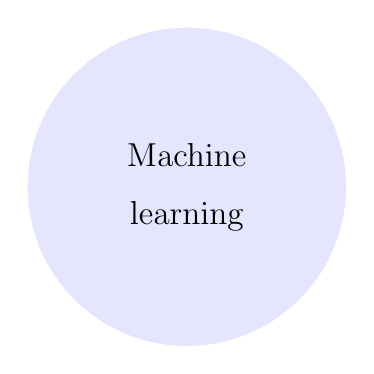
\begin{tikzpicture}
  \path[mindmap,concept color=blue!10,scale=0.3,text width=2.7cm, align=flush center]
    node[concept] {Machine learning};
\end{tikzpicture}

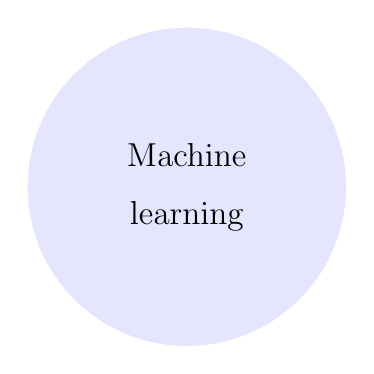
\begin{tikzpicture}
  \path[mindmap,concept color=blue!10,scale=0.1,text width=2.7cm, align=flush center]
    node[concept] {Machine learning};
\end{tikzpicture}

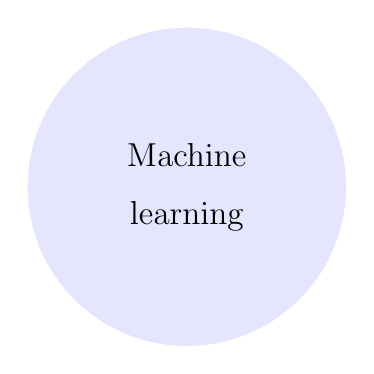
\begin{tikzpicture}
  \path[mindmap,concept color=blue!10,scale=1,text width=2.7cm, align=flush center]
    node[concept] {Machine learning};
\end{tikzpicture}

In practice however a clear separation is often not possible. As such, dimensionality reduction can also be supervised, i.e. labels are provided to learn a new representation of the data \cite{mcinnes2018umap}. Besides, in semi-supervised learning, for example, the goal is the same as for supervised learning. However the data set used to learn the relationship contains both, labeled and unlabeled examples and the hope is to build a stronger representation by providing more information in form of data \cite{Burkov2019}. \\
In addition traditional machine learning is often contrasted to deep learning methods involving the use of artificial neural networks which are composed of many layers of interconnected nodes often used in an end to end fashion in which features are extracted within the network. Usually they require huge amount of data and computational power. In the context of this thesis the tasks considered involve the processing of a \gls{eeg} from experiments with mid to small sample sizes with the goal to learn meaningful patterns and relationships in data. The most commonly used forms in this contexts are supervised and unsupervised learning focusing traditional machine learning. For this reason these forms will be the focus in the following chapters.

\begin{tcolorbox}[breakable, enhanced]
    \subsection*{Excursus: How does a machine learn?}
    "A computer program is said to learn from experience $E$ with respect to some task $T$ and some performance measure $P$, if its performance on $T$, as measured by $P$, improves with experience $E$" \cite{Mitchell1997}. In other words learning in the context of machine learning typically involves solving a specific task by using algorithms that improve their performance by using example data. There are numerous algorithms designed to solve the problems outlined above. Thereby some basic building blocks can be defined which can be used to describe computational learning in a formal way. In the following description the view of statistical learning theory is considered, notation is adapted from \citeauthor{Shalev2014}\cite{Shalev2014}, \citeauthor{Von_luxburg2011}\cite{Von_luxburg2011}.\\
    \\
    Learning always is based on data, i.e. measurable information of some phenomenon, which consists of attributes of the phenomenon, so called features, and in supervised learning an associated label. It can mathematically defined as open bounded set $\mathcal{Z}\subset\mathbb{R}^n$ of dimension $n$. Typically there is only a set of examples or training data $S=\{z_i,...,z_m\}\subset{\mathcal{Z}}^m$ available, where $i = 1,\dots,m$, and each $z_i$ is sampled independently from $\mathcal{Z}$ according to an underlying probability distribution $\mathcal{D}$. Thus the only assumption made is that the example data are independent and identically distributed. No assumption on $D$ is made.\\
    In supervised learning $\mathcal{Z}$ comprises the space of input data $\mathcal{X}$ and the space of labels or output $\mathcal{Y}$. The example data $S$ consists of labeled input-output pairs $z_i=x_i,y_i\in(\mathcal{X}\times\mathcal{Y})^m$, where $x_i$ is an input data vector and $y_i$ is its corresponding output label. The pairs are sampled by some unknown joint probability distribution $\mathcal{D}$ on the space $\mathcal{X}\times\mathcal{Y}$.\\
    The space $\mathcal{Z}$ in unsupervised learning comprises the input data space $\mathcal{X}$ only and the example set $S$ consists of unlabelled examples $z_i=x_i\in\mathcal{X}^m$, sampled according to some unknown probability distribution $\mathcal{D}$ on the space $\mathcal{X}$.\\
    Learning ultimately can be thought of as approximating an underlying ground truth function $f$, also called model, that represents the relationship between input and output in supervised learning, i.e., 
    \begin{equation}
    f:\mathcal{X}\rightarrow\mathcal{Y},
    \end{equation}
    or the mapping to a space of hidden patterns or structure $\mathcal{W}\subset\mathbb{R}^p$, where $p$ can be equal or smaller than $n$, i.e,
    \begin{equation}
    f:\mathcal{X}\rightarrow\mathcal{W}.
    \end{equation}
    A learning task can be conceptualized as searching through the space of all possible solution functions. As this is not feasible a finite class of functions, so called hypotheses, is typically selected a priory. Thus, learning can be thought of as selecting a hypothesis $h$ from a space of potential solutions $\mathcal{H}$ with $\mathcal{H}=\{h:\mathcal{X}\rightarrow\mathcal{Y}\}$ in supervised learning and $\mathcal{H}=\{h:\mathcal{X}\rightarrow\mathcal{W}\}$ in unsupervised learning. \\
    A learner or learning algorithm is the means of selecting the best element from $\mathcal{H}$.
    The cost of a false prediction or an inaccurate representation of the data is quantified using a loss function, $\ell:\mathcal{H}\times\mathcal{Z}\rightarrow\mathbb{R}_+$. In other words it measures how well a specific hypothesis is doing.\\
    The expected risk is measure of the average loss of a hypothesis, $h\in\mathcal{H}$ with respect to the probability distribution $\mathcal{D}$ over $\mathcal{Z}$ and can be defined as
    \begin{equation}
    L_{D}(h):=\mathbb{E}_{z\sim D}[\ell(h,z)]
    \end{equation}
    A learner should select a hypothesis with lowest possible expected risk. However, the underlying probability distribution is unknown. By using $S$ the expected risk can be estimated by using the empirical risk over the training data. This is defined by:
    \begin{equation}
    L_{S}(h):=\frac{1}{m}\sum_{i=1}^m\ell(h,z_i).
    \end{equation}
    Following this, learning can be formalized solving an optimization problem of the form: 
    \begin{equation}
    \hat{h}=\arg\min_{h\in\mathcal{H}}L_{S}(h),
    \end{equation}
    which can be solved computationally. In parameterized models, this often involves the automated selection of those parameters $\theta\in\Theta$ of a chosen class of models that minimize $L_{S}(h_\theta)$. This optimization problem can then be solved by various methods such as gradient descent, or e.g., analytically using least squares estimation. The solution $\hat{h}$ is the learned model that can be used to solve the task at hand, e.g. predicting the label of new input data or uncovering patterns or structure in data. This is known as \gls{erm}.\\
    Upon \gls{erm} more complex learning paradigms can be used addressing common problems such as overfitting, in which the learned hypothesis to closely relies on the training data and therefore has low generalization performance, e.g. regularized risk minimization which introduces regularization to \gls{erm} or structural risk minimization that penalizes complex models and encourages simplicity.\\
    \\
    Although most machine learning can conceptualized within the framework of \gls{erm} there are models that instead of minimizing risk assume that the underlying distribution over the data has a specific parametric form and the goal is to estimate these parameters by using \gls{mle} which seeks to find the model parameters that maximize the likelihood of the observed data under the assumed parametric distribution, i.e. \\
    \begin{equation}
    \hat{\theta}_{\text{MLE}} = \arg\max_{\theta\in\Theta}\prod_{i=1}^{m}p_{\theta}(z_i),
    \end{equation}
    where $p_{\theta}(z)$ is the joint probability function of the assumed parametric distribution and $\hat{\theta}_{\text{MLE}}$ is the estimated value of the parameter vector $\theta$.
\end{tcolorbox}

\subsection{Applications in the context of aging research}
Traditionally, machine learning has been the core building block for the development of intelligent systems that can automate tasks or enhance and assist humans in performing their tasks. Such systems are not only important in terms of assistive technology, for example to support elderly people with disabilities to live their daily lives, but are also relevant in the medical fields. In the latter the hope is to develop intelligent medical systems to inform clinical theory and support clinical decision making, i.e. assist in diagnosis, and risk management by predicting health status or forecasting of treatment responses \cite{Woo2017}. In this context, supervised learning is often used to identify markers from \gls{eeg} by identifying signal features that are predictive of a particular disease or health condition, which is highly important in terms of promoting a healthy aging trajectory \cite{Babiloni_AlzCons2021,Mei2021}. An application is the estimation of biological age based on regression models trained on the basis on neural data, e.g. \gls{eeg} data, recorded in large population studies \cite{Engemann2022}. Using data of an individual person, a regression model can predict the age of that person. If the brain appears older than it would chronologically, this can be an early indication of an unfavorable state of health \cite{Gonneaud2021}.\\
Another in the context of aging highly relevant application is the development of devices with the goal to assist, augment or enhance humans capabilities such as \glspl{bci}. In \glspl{bci}, neural activity is decoded, using classification to generate control commands for various external devices such as computers or prosthetic limbs \cite{Saha2021, Anumanchipalli2019}. Decoding hereby refers to learning a classification or regression model that is capable of predicting behavioral outcomes or cognitive states based on neural data.\\
\\
Beyond the application in \glspl{bci}, decoding techniques are widely used in neuroscientific research to gain insights into the neural mechanisms underlying perception, cognition, and behavior. This type of analysis is often referred to as \gls{mvpa} because its goal is to detect multivariate patterns, e.g., a set of voxels in \gls{fmri} or an electrical pattern at a given time point in \gls{eeg}, associated with an experimental condition \cite{Holdgraf2017}. While the use has a long history in the field of \gls{fmri} analysis, it has only become more widespread in the field of \gls{eeg} in recent years.  Therefore, decoding approaches to understand age-related reorganization are mostly limited to fMRI studies. A common approach is to measure dedifferentiation, i.e. the loss of neural specificity, at the individual level. Since dedifferentiation by definition results in more similar brain activation patterns for different tasks or stimuli, poorer performance of classifiers trained to discriminate between them based on neural recordings is indicative of a less distinctive neural representation \cite{Koen2019, Park2010}. \\ 
Furthermore, the classification of group membership or group level regression can provide information about interesting relationships and their generalizability. Particularly for \gls{eeg} markers representing functional network characteristics can reveal insightful findings about the relationship to age-related changes \cite{Petti2016}.\\
In addition to the application of supervised learning algorithms, unsupervised learning algorithms have long been used in neuroscience. Unsupervised methods are often used as a preprocessing step to reduce the complexity of \gls{eeg} data but can also provide interesting insights into the structure of data sets. Dimensionality reduction algorithms can provide insights into high-dimensional data by providing a possibility to visualize high dimensional patterns of \gls{eeg} data \cite{Kottlarz2020, Banville2021}. This can be used to study the temporal structure of \gls{eeg} signals in terms of the dynamic of brain networks with aging \cite{Brunton2016, vieluf2018age}.\\
\\
In summary, the use of machine learning is very diverse and ranges from engineering applications to scientific knowledge discovery. Especially in the latter case, it offers the advantage of automated extraction of patterns from highly complex data that can contribute to the study of age-related changes. While decoding approaches are particularly interesting for measuring age-related changes in the organization of neural systems, such as the level of differentiation, group analysis could provide new insights into datasets. Especially classification methods that allow to predict a certain experimental condition or a group membership are particularly suitable. The combination with unsupervised learning algorithms such as dimensionality reduction methods could be particularly beneficial and used for the visualization of high-dimensional data. Based on this, the next section will present common approaches with a focus on the classification and dimensionality reduction of EEG data.

\subsubsection{State of the art approaches}
Selecting a suitable learning algorithm for classification, i.e. classifier, involves an iterative approach that divides the available data into training and testing sets, trains and validates various classifiers within the training portion (cross-validation), and finally tests the best performing model on the testing portion to estimate its ability to generalize \cite{Hastie2009}. Different classifiers may have varying strengths and weaknesses, with popular examples including \glspl{svm}, \gls{lda}, and \glspl{rf} (see \cite{shoorangiz2021eeg} for an overview).\\
While deep neural networks are capable of learning on the basis of raw data their advantage comes into play with large labeled data resources, which are often expensive to acquire in the case of \gls{eeg} \cite{Banville2021}. Traditional learning approaches can be more efficient with good performance and promise better interpretability, especially for comparatively smaller data sets and limited computational resources \cite{Gemein2020}. Due to the low signal-to-noise ratio and high complexity of \gls{eeg} data, the inputs in these approaches are typically represented by well known \gls{eeg} characteristics, or features, that are believed to be related to the problem being learned. Typical features include parameters of time, frequency, time-frequency, connectivity and information theoretical parameters extracted for each sensor (see \cite{Gemein2020} for common choices). However, this approach may lead to less flexible and generalizable models with low spatial resolution and vulnerability to low signal-to-noise ratios \cite{Saeidi2021}.\\
To address this, some approaches compute the sources of the \gls{eeg} signals in the brain using biophysical models as a preprocessing step prior to feature extraction \cite{Khan2018, Westner2018}. Other approaches use supervised and unsupervised decomposition techniques belonging to the field of dimensionality reduction as a preprocessing step for further prediction tasks or provide information themselves in the sense of knowledge discovery. These methods aim at \textit{unmixing} the highly correlated sensor time series by assumptions about the underlying signal components. For example, \gls{ica} assumes statistical independence, while \gls{pca} assumes that the extracted components are maximally uncorrelated to each other, capturing the largest amount of variance in the data \cite{CohenX2017}. \Gls{dmd} is a method that explicitly considers the temporal structure of the signals, which requires the extracted signal patterns (modes) to be temporally coherent, thus accounting for the network character of the brain \cite{Brunton2016}. Additionally, supervised methods such as \gls{csp} \cite{Blankertz2008} or xDAWN \cite{rivet2009xdawn} extract signal components that correlate with the labels to be predicted.\\
While supervised and unsupervised ways of examining the complex \gls{eeg} signals in terms of components and patterns to generate knowledge, non-linear methods such as \gls{tsne} and \gls{umap} take into account the non-linear relationships between the data points and provide a lower-dimensional representation of the data that is often easier to interpret and visualize \cite{mcinnes2018umap}. These methods can be particularly useful for exploring the relationships between different \gls{eeg} features or for identifying subgroups within a dataset.\\
It is important to note that these methods can be applied not only to the \gls{eeg} signals itself, but also to previously extracted \gls{eeg} parameters or in combination in terms of knowledge discovery. Thus, supervised and unsupervised dimension reduction provides data-driven insights into the complex underlying information, but also serves as preprocessing for further tasks such as prediction. Figure \ref{fig1:ml_approoaches} summarizes these common approaches.

\begin{figure*}[h]
  \dummyfig{Typical cross validation workflow } 
  \caption{State of the art approaches}
  \label{fig1:ml_approoaches}
\end{figure*}

 
    
\chapter{Aims and scope}
\label{chap:aims_scope}
The overall goal of my dissertation is to apply previously presente methods from supervised and unsupervised machine learning to \gls{eeg} signals in order to capture the age-related reorganization of the brain both in terms of overreaching patterns as well as individual trajectories. This is done by using data sets that include subjects at different life stages including influencing factors such as professional expertise and physical fitness. In four empirical studies it will be investigated how the reorganization of the brain can be detected based on \gls{eeg} data and how factors contributing to reserve such as professional expertise or physical activity can be characterized using supervised and unsupervised machine learning. In detail the following research questions will be answered.\\
\\
\textit{How can the reorganization of the brain be detected based on \gls{eeg} data using supervised and unsupervised machine learning algorithms?}\\
\\
\textit{How do professional expertise and physical activity affect the reorganization of the brain, and can these factors be characterized based on \gls{eeg} data using machine learning techniques?}\\
\\
\textit{Can machine learning algorithms accurately differentiate between individuals with different levels of professional expertise based on \gls{eeg} data, and what are the key features of the EEG data that contribute to this differentiation?}\\
\\
\textit{How does physical fitness affect the brain's reorganization over time, and can this be detected based on changes in EEG data using machine learning techniques?}\\
\\
The application of supervised machine learning methods both on individual as well as group level, as well as dimensionality reduction methods, will allow to draw conclusions about predictors of reorganization of brain networks and will help to identify the individual status as well overreaching trajectories. The information gained from these tools could be usedto determine and evaluate intervention programs, on-the-job-trainings, support diagnosis, and may have applications in the development on assistive technological systems. 

\chapter{General methodology}
\label{chap:methods}
% To approximate the performance of a predictive model a dataset is typically divided into a training and testing set. The training set is used for learning a model whereas the testing set is used to estimate the generalization performance to new unseen data, i.e. data which was not used during the process of training. The training data can further be divided into a training and validation portion in order to compare different model types or user defined settings of a learning algorithms, so called hyperparameters. However, this three time division may drastically reduce the data size usable for training and my result in flawed generalization evaluation due to the randomness of the split. Therefore several procedures can be applied. In a simple k-fold cross-validation, for example, the training data is divided k-times. Thus each time a different subset of the data is used for validation while the rest is used for training. Usually this is repeated for a range of models and subsequent hyperparamters and the model and hyperparameter performing best on average are selected for final testing. A more advanced method denoted nested cross-validation adds a second k-fold cross-validation loop for the final model evaluation (see Figure \ref{fig1:CV} for a visual representation of the procedures).    

% \begin{figure*}[h]
%   \dummyfig{Cross-validation procedures} 
%   \caption{Cross-validation procedures}
%   \label{fig1:CV}
% \end{figure*}


\chapter{Results}
\label{chap:results}
    \section{Paper 1}
    \label{results:paper1}

    \section{Paper 2}
    \label{results:paper2}

    \section{Paper 3}
    \label{results:paper3}

    \section{Paper 4}
    \label{results:paper4}
    
\chapter{General discussion}
\label{chap:discussion}

\printbibliography
\end{document}